% !TeX spellcheck = cs_CZ
%{\tikzset{external/prefix={tikz/FYZI/}}
% \tikzset{external/figure name/.add={ch31_}{}}
%=========================== Kapitola: Původ indexu lomu ==========================================
\chapter{Původ indexu lomu}\label{fyz:IchapXXXI}
\minitoc
  \section{Index lomu}\label{fyz:IchapXXXIsecI}
  \section{Pole v látce}\label{fyz:IchapXXXIsecII}
  \section{Disperze}\label{fyz:IchapXXXIsecIII}
  \section{Absorpce}\label{fyz:IchapXXXIsecIV}
  \section{Energie přenášená elektrickou vlnou}\label{fyz:IchapXXXIsecV}
  \section{Difrakce světla na cloně}\label{fyz:IchapXXXIsecVI}
  \section{Příklady a cvičení}\label{fyz:IchapXXXIsecVII}

    \begin{figure}[ht!] %\ref{fyz:fig261}
      \centering
      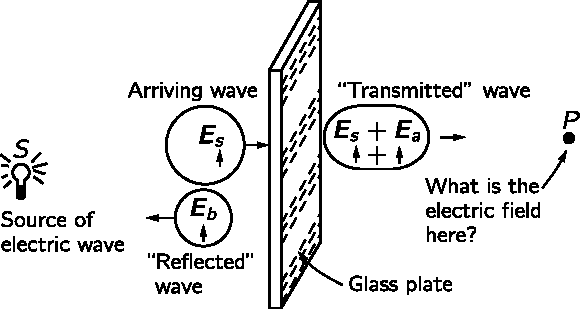
\includegraphics[width=0.9\linewidth]{fyz_fig261.pdf}
      \caption{Elektromagnetická vlna při průchodu vrstvou průhledné látky
               (\cite[s.~411]{Feynman01})}
      \label{fyz:fig261}
    \end{figure}

    \begin{figure}[ht!] %\ref{fyz:fig262}
      \centering
      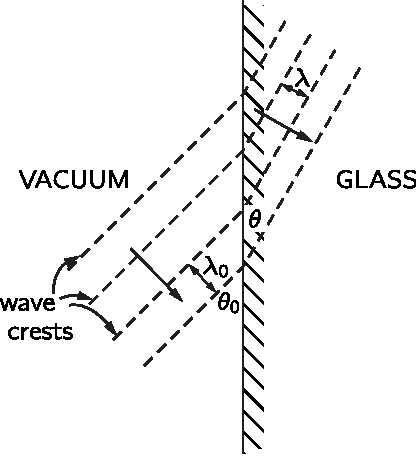
\includegraphics[width=0.9\linewidth]{fyz_fig262.pdf}
      \caption{Vztah mezi lomem vln a změnou jejich rychlosti
               (\cite[s.~412]{Feynman01})}
      \label{fyz:fig262}
    \end{figure}

    \begin{figure}[ht!] %\ref{fyz:fig263}
      \centering
      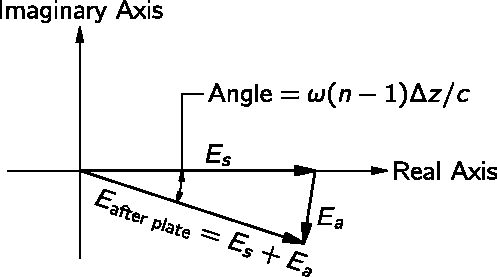
\includegraphics[width=0.9\linewidth]{fyz_fig263.pdf}
      \caption{Graf k určení prošlé vlny pro dané \(t\) a \(z\)
               (\cite[s.~413]{Feynman01})}
      \label{fyz:fig263}
    \end{figure}
    
    \begin{figure}[ht!] %\ref{fyz:fig264}
      \centering
      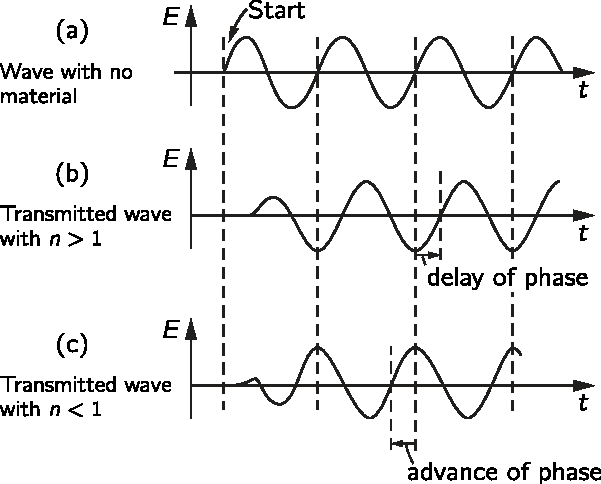
\includegraphics[width=0.9\linewidth]{fyz_fig264.pdf}
      \caption{Vlnové signály
               (\cite[s.~418]{Feynman01})}
      \label{fyz:fig264}
    \end{figure}

    \begin{figure}[ht!] %\ref{fyz:fig265}
      \centering
      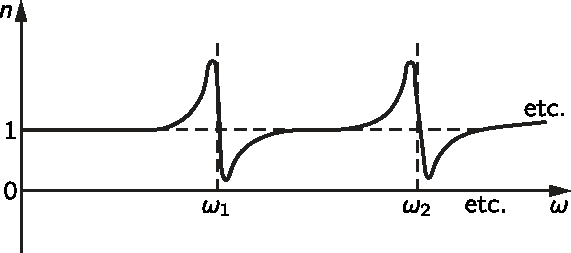
\includegraphics[width=0.9\linewidth]{fyz_fig265.pdf}
      \caption{Index lomu jako funkce frekvence
               (\cite[s.~419]{Feynman01})}
      \label{fyz:fig265}
    \end{figure}
    

    \begin{figure}[ht!]  %\ref{fyz:fig266}
      \centering
      \begin{tabular}{c}
        \subfloat[ ]{\label{fyz:fig266a}
          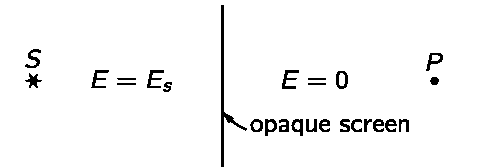
\includegraphics[width=0.7\linewidth]{fyz_fig266a.pdf}}               \\
        \subfloat[ ]{\label{fyz:fig266b}
          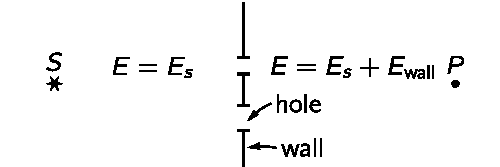
\includegraphics[width=0.7\linewidth]{fyz_fig266b.pdf}}               \\
        \subfloat[ ]{\label{fyz:fig266c}
          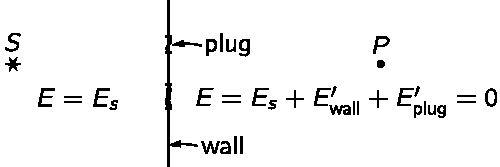
\includegraphics[width=0.7\linewidth]{fyz_fig266c.pdf}}
      \end{tabular}
      \caption{Difrakce na stínítku
               (\cite[s.~422]{Feynman01})}
      \label{fyz:fig266}
    \end{figure}

%} %tikzset
%---------------------------------------------------------------------------------------------------
\printbibliography[title={Seznam literatury}, heading=subbibliography]
\addcontentsline{toc}{section}{Seznam literatury}